\title{Simulation using Hamiltonian Monte Carlo}
\author{
        Ho Chung Leon  Law \\
            \and
        Nathan Cunningham\\
}
\date{\today}

\documentclass[11pt]{article}
\usepackage{amsmath}
\usepackage{algorithm}
\usepackage{algpseudocode}
\usepackage{graphicx}
\usepackage{amssymb}
\usepackage{hyperref}
\usepackage[a4paper,bindingoffset=0.2in,%
            left=1in,right=1in,top=1in,bottom=1in,%
            footskip=.25in]{geometry}
\begin{document}
\maketitle

\begin{abstract}
\noindent In this report we aim to examine the properties of Hamiltonian Monte Carlo, implement it in R and compare its effectiveness against other MCMC samplers. We also provide a R package that implements HMC, random walk Metropolis Hastings and also samples from a mixture of bivariate gaussians that resemble letters, which were constructed by using the EM algorithm.   
\end{abstract}
\newpage
\section{Introduction}
Popular methods to simulate from a density of interest include Random Walk Metropolis-Hastings and Gibbs Sampling, however, these may have slow mixing properties, especially in a high-dimensional setting. Hamiltonian Monte Carlo (HMC) can overcome this by making use of first-order gradient information of the target density and Hamiltonian dynamics, which allows us to coherently explore the state space. This is done through the introduction of auxiliary momentum variables, which allows the use of Hamiltonian dynamics to construct a Markov chain, whose stationary distribution is our density of interest. 
\\
\\
In this report, we will first give a quick overview and intuition of the HMC algorithm, which is primarily based on Neal \cite{neal} and Duane et al \cite{duane}. We will then go on to implement the algorithm in R and compare results to those obtained from different samplers, such as random walk Metropolis Hastings and No-U-Turn Sampler (NUTS). We will also illustrate these methods on bivariate Gaussian mixture models, whose densities represent the 26 letters of the alphabets (upper and lower case), where the parameters were found by using the EM-algorithm on an image data set of the letters of the alphabet using the R package $mixtools$. Our code is collated in the R package ``abcHMC" and basic instructions are given at the end.
\section{Hamiltonian Monte Carlo}
\subsection{Hamiltonian dynamics}
We will begin by describing Hamiltonian dynamics, before stating how we will utilise them in the next section. Hamiltonian dynamics is the system described by a pair of differential equations with coordinates $(\mathbf{q},\mathbf{p}) \in \mathbb{R}^{2d}$.\\ For $i=1 \dots d$,
\begin{equation}
\label{Ham1}
\frac{dq_{i}}{dt} = \frac{\partial H}{\partial p_{i}}
\end{equation}
\begin{equation}
\label{Ham2}
\ \ \frac{dp_{i}}{dt} = -\frac{\partial H}{\partial q_{i}}
\end{equation}
where $H$ is called the Hamiltonian and is a function of time and $(\mathbf{q},\mathbf{p})$. This system arises from Newtonian Mechanics, and has a natural interpretation in physics. If we think of $(\mathbf{q}(t),\mathbf{p}(t))$ as 2-dimensional position and momentum  vectors at time t, respectively, and the Hamiltonian as simply the sum of the kinetic (function of $\mathbf{p}$) and potential energy (function of $\mathbf{q}$), we can just think of the equations as describing the evolution of a particle over time through a frictionless system. We will now set up our notation and the introduce the idea of an energy function.
\subsection{Target Density and Energy Function}
We first define our target density to be of the form (without normalising constant):
\begin{equation}
P(\mathbf{q})= \pi(\mathbf{q})L(\mathbf{q}|D) \quad \quad q \in \mathbb{R}^{d}
\end{equation}
where $\pi(\mathbf{q})$ is the prior density and $L(\mathbf{q}|D)$ is the likelihood given data $D$. 
We also define $\mathbf{q}$ to be the `position' vector in $d$ dimensions. Now, from statistical mechanics, given some energy function $E(x)$ in some system, we can express its canonical distribution as:
\begin{equation}
\label{energy}
Pr(x) = \frac{1}{N}\exp(-E(x)/T)
\end{equation}
where $T$ is the temperature of the system (assumed to be 1) and $N$ is a normalising constant. By considering this, we can define the energy of our target density as:
\begin{equation}
U(\mathbf{q}) = -\log [\pi(\mathbf{q})L(\mathbf{q}|D)]
\end{equation}
We now introduce an auxiliary variable $\mathbf{p}$ (which we denote as `momentum' in $d$ dimensions), which we define to have energy function $K(\mathbf{p})$, which using equation (\ref{energy}) has in turn a density function $Q(\mathbf{p})$ say. We then define the joint density of $(\mathbf{q},\mathbf{p})$ with normalising constant $Z$ as 
\begin{equation}
\label{joint}
P_{\text{joint}}(\mathbf{q},\mathbf{p}) = \frac{1}{Z}\exp(-U(\mathbf{q})/T)\exp(-K(\mathbf{p})/T) = \frac{1}{Z}\exp(-H(\mathbf{q},\mathbf{p})/T)
\end{equation}
where $H(\mathbf{q},\mathbf{p}) = U(\mathbf{q}) + K(\mathbf{p})$ now can be seen as the energy function for the joint state $(\mathbf{q},\mathbf{p})$ distribution. The construction of independence between $\mathbf{q}$ and $\mathbf{p}$ may seem meaningless at first, but this introduction enables us to use Hamiltonian Dynamics, which has properties crucial to our construction of the Markov chain. This independence of $\mathbf{q}$ and $\mathbf{p}$ also allows us to easily extract samples with respect to $P(\mathbf{q})$.

\subsection{Properties of Hamiltonian dynamics}
We will now briefly state several important properties of the Hamiltonian, which are crucial to the HMC algorithm, before stating the relationship between the dynamics and our $P(\mathbf{q},\mathbf{p})$ density. Firstly, the the dynamics keeps the Hamiltonian invariant, i.e. the Hamiltonian remains constant, this means the mapping $T_s: (\mathbf{q}(t),\mathbf{p}(t)) \rightarrow (\mathbf{q}(t+s),\mathbf{p}(t+s))$, where the arrow represents the evolution of the system is independent of time. This brings us to the second property, which says that the mapping $T_s$ is reversible, in the sense that it is a one-to-one mapping. This reversible property is important to show the Markov chain constructed in Algorithm 1 satisfies detailed balance and hence leave the desired distribution invariant. The third important property is that Hamiltonian dynamics preserves volume in the $(\mathbf{q},\mathbf{p})$ space, in the sense that the image of $T_s$ from some region R has the same volume as region R. This property means that there is no need to account for any change in volume in the acceptance probability of Metropolis Hastings, where for general dynamics will be infeasible to compute. To understand these exact properties, see \cite{neal}.
\subsection{Hamiltonian Dynamics and Hamiltonian Monte Carlo}
Because of these nice properties of the Hamiltonian dynamics, we may like to construct a Hamiltonian and Markov chain that make use of these properties. This is exactly our $H(\mathbf{q},\mathbf{p})$ we defined earlier in equation (\ref{joint}), where we have introduced an `momentum' variable $\mathbf{p}$. Looking at the form of the Hamiltonian, we can in fact attach our previous physical interpretation of `potential' ($U(q)$) and `kinetic' energy ($K(p)$) to it. 
\\
\\
As an illustration, let $P(q)$ be a univariate Gaussian, which means that $U(q)=\dfrac{q^2}{2}$. So imagine putting a particle on the energy function of this gaussian and giving it some momentum in some direction, then Hamiltonian dynamics is then exactly describing the transfer of energy between $U(q)$ and $P(q)$, as the Hamiltonian is conservative. So given sufficient energy, the particle will in fact `travel' a sufficiently `large' amount of the state space of the position vector $q$ in some time period. HMC basically make use of this by constructing a new position state from the previous position state by stopping the dynamics after initialising from previous position state and some random momentum. It is important to note here, unlike proposals in Random Walk Metropolis Hastings, due to the properties of the Hamiltonian, the acceptance probability of this new state is always 1. 
\\
\\
This allows for coherent exploration of the state space, and in fact this exploration can be thought of as travelling along the contours of the $-\log P(\mathbf{q},\mathbf{p})$ or equivalently the Hamiltonian energy function $H(\mathbf{q},\mathbf{p})$ due to the conservation of the Hamiltonian dynamics and the `jump' between the contours of the energy levels is done by sampling momentum with respect to the corresponding density function of $K(\mathbf{p})$. This replacement of $\mathbf{p}$ can change the probability density of $(\mathbf{q},\mathbf{p})$ by a large amount, hence also for $P(\mathbf{q})$, allowing exploration.
\\
\\
We have yet to specify the energy function $K(\mathbf{p})$, but in theory most positive functions can be chosen. A common choice is to use the energy function from a multivariate Gaussian with mean $\mathbf{0}$ and diagonal covariance matrix $\mathbf{M}$, with $m_{i}$ along the diagonals.
\begin{equation}
K(\mathbf{p}) = \sum_{i=1}^{d} \frac{p_{i}^{2}}{2m_{i}}
\end{equation}
This is chosen because: the Gaussian distribution can be easily sampled from; it is only intuitive to choose a symmetric density with an infinite support to encourage mixing of the chain; and this has an interpretable physical analogue, being exactly the kinetic energy form we observe in nature. 
\subsection{The Leapfrog}
In general, a solution to the Hamiltonian dynamics given by an arbitrary Hamiltonian of the form $H(\mathbf{q},\mathbf{p}) = U(\mathbf{q}) + K(\mathbf{p})$ cannot be computed analytically. Hence, we discretise the time in equation (\ref{Ham1}) and (\ref{Ham2}) with some small step size $\epsilon$ and we approximate the solution to the equations using the leapfrog method:
\\ For $i=1\dots d$, first advance the momentum by one half-step:
\begin{equation}
p_{i}(t+\epsilon/2) = p_{i}(t) - (\epsilon/2)\frac{\partial U}{\partial q_{i}}(\mathbf{q}(t))
\end{equation}
then advance the position by a full-step using the updated momentum:
\begin{equation}
q_{i}(t+\epsilon) = q_{i}(t) - (\epsilon)\frac{p_{i}(t+\epsilon/2)}{m_{i}}
\end{equation}
And finally advance the momentum one half-step using the updated position:
\begin{equation}
p_{i}(t+\epsilon) = p_{i}(t+\epsilon/2) - (\epsilon/2)\frac{\partial U}{\partial q_{i}}(\mathbf{q}(t+\epsilon))
\end{equation}
Iterating over this process $L$ times simulates the dynamics for a time of $L\epsilon$.
Note this method in fact preserves volume exactly, as each step is just a shear transformation, and furthermore it is also reversible, by simply negating p and reapplying the steps. For more details on the local and global error and comparison to Euler's Method, see \cite{neal}.
\\
\\
Although the volume is conserved exactly, the value of Hamiltonian is not conserved exactly, due to the approximate error introduced by discretising. However, we will see later that this can easily be fixed using a Metropolis-Hastings step. Commonly, there exists a critical step size, where above this value, the error of the Hamiltonian can grow without bound and below this value, the error tends to stay bounded regardless of size of $L$. Hence, it is important to observe the change in the Hamiltonian or the acceptance rate of the process in order to tune the size of $\epsilon$ and $L$. It is also important to note that we must be able to compute the partial derivatives of the log of the density function we are interested in, and some R packages such as RStan\cite{rstan} provide a way to do this.
%It is important to note that the particle will tend to travel in some direction, before making a u turn to come back, 

% is fact just a reformulation of Newtonian Mchanics (Newton's Laws). If we now think of 
%The Hamiltonian equations model the evolution of a particle in a frictionless system over time, $t$, given its momentum, $p$, and position, $q$. The Hamilton equation consists of the potential energy of the particle, $U(q)$, and the kinetic energy, $K(p)$, and in Hamiltonian Monte Carlo is usually written as


%Thus, we can convert our distribution $P(x)$ to a canonical distribution by setting the energy function, $E(x)$ to $-logP(x)-logZ$
\pagebreak
\subsection{The Hamiltonian Monte Carlo Algorithm}
We will now present the HMC algorithm and give some intuition behind the steps. The R package ``AbcHMC" includes an implementation of this algorithm. 
\begin{algorithm}
\caption{Hamiltonian Monte Carlo}\label{euclid}
\begin{algorithmic}[1] 
\State Select an initial $\mathbf{q}$ 

\State $\mathbf{p}\sim \mathcal{MN}(\mathbf{0},\mathbf{M})$
\State Given $(\mathbf{q},\mathbf{p})$, simulate Hamiltonian dynamics using the leapfrog for $L$ steps with $\epsilon$ to find $(\mathbf{q^{*}},\mathbf{p^{*}})$ 
\State Negate $\mathbf{p^{*}}$ to ensure reversibility 
\State Accept $(\mathbf{q^{*}}, \mathbf{p^{*}})$ as the next step in the Markov chain with probability M given below, otherwise accept $(\mathbf{q},\mathbf{p})$ as next state.
\State Return to step 2 with new state for next simulation.
\end{algorithmic}
\end{algorithm}\\
\noindent There are 2 main steps to the algorithm, the sampling of the momentum and the Metropolis update with a Leapfrog proposal. All these steps leave the joint distribution of ($\mathbf{q}$,$\mathbf{p}$) invariant, and hence their combination also leave the distribution of interest invariant. In step 2, new momentum is simulated from the multivariate gaussian distribution, where commonly $\mathbf{M}$ is just the identity matrix. Due to the independence of $\mathbf{q}$ and $\mathbf{p}$ from our construction, the marginal density of $\mathbf{p}$ is exactly the conditional distribution given $\mathbf{q}$, this is in fact just a Gibbs update, and clearly this leaves the joint distribution invariant. 
\\
\\
In step 3, we propose a new state $(\mathbf{q^{*}},\mathbf{p^{*}})$ by simulating Hamiltonian dynamics using Leapfrog with L steps and $\epsilon$ step size. The negation of momentum in step 4 ensures reversibility, although in practice this negation needs not be done as $K(\mathbf{p})=K(-\mathbf{p})$ and momentum will always be resampled in the next iteration. If we simulated the Hamiltonian dynamics perfectly, then we would always accept the new state, as we are travelling on the contours on the $(\mathbf{q},\mathbf{p})$ energy/density space, where the Hamiltonian is constant. However, due to approximation error, the Hamiltonian will not be conserved exactly, hence we will use Metropolis to correct for this, where the new state $(\mathbf{q},\mathbf{p})$ is accepted as the next state of the Markov chain with probability
\begin{equation}
M=\min \{1,\exp(-H(\mathbf{q^{*}},\mathbf{p^{*}})+H(\mathbf{q},\mathbf{p}))\} = \min\{1, \exp(-U(\mathbf{q^{*}})+U(\mathbf{q})-K(\mathbf{p^{*}})+K(\mathbf{p}))\}
\end{equation}
Note that this is just the normal Metropolis step on $(\mathbf{q},\mathbf{p})$ written in terms of the energy form. This means that a large difference in approximation error of the Hamiltonian  will in turns give a large chance of rejection, hence we can see that some tuning will be necessary to encourage mixing of the chain. The properties of Hamiltonian dynamics means that detail balance will hold and hence leave the canonical distribution of the constructed Markov Chain invariant. For more information, refer to \cite{neal}.

\subsection{Ergodicity and the choice of $L$ and $\epsilon$}
The HMC method is sensitive to the user-tuned parameters $L$ and $\epsilon$, and in fact if the solution to the equations (\ref{Ham1}) and (\ref{Ham2}) are periodic, and if $L\epsilon$ is close to this period, then trajectories from the Leapfrog will return proposals that are close to the original $\mathbf{q}$, and hence the HMC may not give an ergodic Markov Chain. One way of solving this is to randomly choose $L$ and $\epsilon$ from some small interval routinely. 
\\
\\
Choosing $L$ and $\epsilon$ is also a major issue in HMC, as for a small value of $L$, the algorithm devolves to random walk behaviour, since the position of the particle will be very dependent on the initial momentum. As going back to the previous example, where $P(q)$ is a univariate Gaussian, given some position on the energy function, for a small interval of time, the particle will basically move according to the direction of the momentum and also unlikely to move far from the starting position. This is exactly like  a random walk behaviour, and hence the samples are likely to be highly correlated. For L too large, it is computationally wasteful as the particle might have a performed a `U turn' and extra work is being done to propose a $\mathbf{q^{*}}$ that is close to our original $\mathbf{q}$. The value of $\epsilon$ affects our error in the Hamiltonian and could lead to a high rejection rate if $\epsilon$ is too big, however too small $\epsilon$ means extra leaps will be needed to explore further, wasting computational power. The choice of $L$, $\epsilon$ and even $\mathbf{M}$ takes experiences, requiring preliminary runs with different values of $L$ and $\epsilon$. A lot of work has been done since to attempt to automate this tuning of parameters, with one important example being the No U-turn sampler (NUTS).
\subsection{No U-turn sampler (NUTS)}
The No U-turn sampler\cite{NUTS} is an implementation of an algorithm based on Hamiltonian Monte Carlo which aims to avoid the need for the user to manually specify $L$ and $\epsilon$. To find the number $L$ of leap frog steps, it uses a criterion based on half the squared distance between initial position $\mathbf{q}$ and $\mathbf{q^{*}}$:  
\begin{equation}
\frac{d}{dt}\frac{(\mathbf{q^{*}}-\mathbf{q}) \cdot(\mathbf{q^{*}}-\mathbf{q}) }{2}=(\mathbf{q^{*}}-\mathbf{q})\frac{d}{dt}(\mathbf{q^{*}}-\mathbf{q})=(\mathbf{q^{*}}-\mathbf{q})\cdot \mathbf{p^{*}}
\end{equation}
This suggests that an algorithm that runs leapfrog steps until the dot product between the current momentum and $\mathbf{q^{*}}-\mathbf{q}$ becomes less than $0$ would simulate system's dynamics until a `U turn' occur and it starts to move back to $\mathbf{q}$, meaning that computational power would not be too wasted or $L$ number of leaps will not be too small. However, this does not guarantee time reversibility, but NUTS uses a recursive algorithm involving trees and repeated doubling to overcome this issue. NUTS also adapts the step size $\epsilon$ on the fly based on primal-dual averaging. For more information, please refer to \cite{NUTS}.
\section{Comparisons between HMC, MH and NUTS}
\subsection{Bivariate Gaussian simulation}
We begin by illustrate the HMC method on a bivariate Gaussian with mean $(0,0)$ and standard deviations of 1 and correlation of $0.95$. For HMC, a value of $\epsilon$ of $0.20$ and $L=25$ was chosen by looking at auto-correlation and trace plots, such that the `particle' was able to travel to a sufficiently distant point, independent of the previous point. If we examine the dynamics of the each step of the leap-frog from the starting position at say $\mathbf{q}=(-2,-2)$, we should see that most of the dynamics will be travelling in one direction, which is consistent with our interpretation of equation (\ref{Ham1}) and (\ref{Ham2}). In figure 1, we can see that the samples from the HMC travels a significantly large part of the state space and are relatively independent of the last state. Also, the rejection rate of the sample is 0 in this case, as the step size is relatively low. This is unlike in a random walk Metropolis (proposal of $U[-0.25,0.25]$ around current state) where even after a thinning of 25 samples, it still exhibits a highly auto-correlated behaviour and the rejection rate around 0.4. However, the computational efficiency of both samplers on large samples has yet to tested, since proper comparisons on R is difficult.
\begin{figure}[H]
\center
  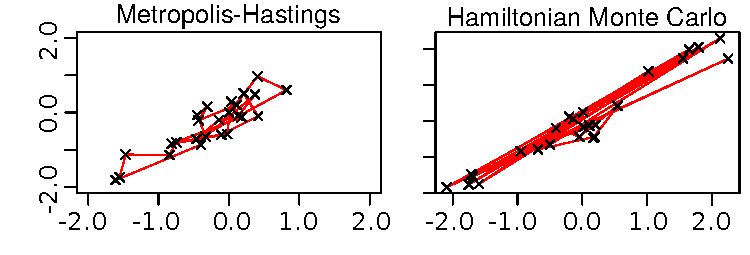
\includegraphics[width=5in]{images/MHvsHM_explore.pdf}
\caption{The trajectory of a bivariate Gaussian distribution simulated with zero-mean and marginal $\sigma$ of 1, and correlation of 0.95.}
\end{figure}
\subsection{High-dimensionality}
We will now illustrate the behaviour of random-walk Metropolis, HMC and NUTS on a 150 dimensional independent multivariate gaussian with means of 0 and increasing standard deviation of approximately 0.0065 step from 0.02 to 1. For the HMC, it was tune to have $\epsilon = 0.014$ and $L=100$, from examinations of the rejection rates and diagnostic plots and also understanding that the step size is limited by the small standard deviation. Since such a small step size was chosen, it was necessary to choose a sufficiently large leap size in order to move sufficiently in the direction of large standard deviation. To avoid any possible problem with periodicity, the $\epsilon$ was randomised uniformly on $0.014 \pm 20 \%$. Random walk Metropolis was also used with proposals generated from $U[0.02,0.03]$ with a thinning of 100 samples to roughly compare the computational time. The rejection rate was 0.5 for the Metropolis Hasting and 0.05 for the HMC algorithm. 
\\
\\
\begin{figure}[H]
\center
  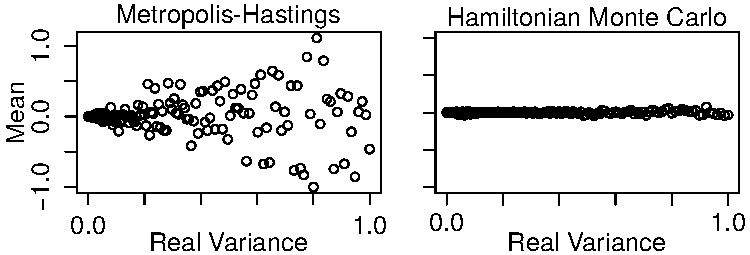
\includegraphics[width=5in]{images/MHvsHM_var.pdf}
  \caption{Sample Mean against the Real Variance of a multivariate gaussian in 150 dimensions with 1000 samples}
\end{figure}

\begin{figure}[H]
\center
  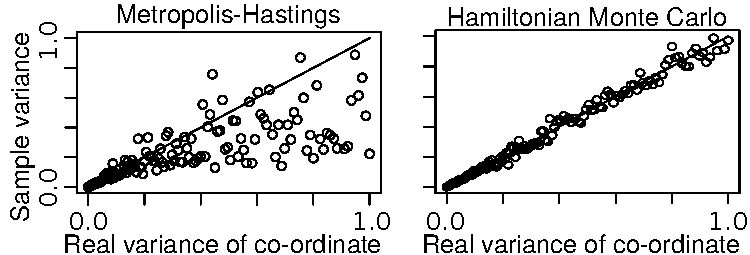
\includegraphics[width=5in]{images/MHvsHM_varcoord.pdf}
  \caption{Sample Variance against the Real Variance of a multivariate gaussian in 150 dimensions with 1000 samples}
\end{figure}
\noindent From looking at different trace and auto-correlation plots for different variables, one can clearly see much higher correlation between samples in the random walk Metropolis compared to that of HMC. Figure 2 and Figure 3 shows the sample mean and sample variance of the 1000 samples obtained from HMC and Metropolis, clearly here HMC outperforms MH. Further experimentation can show that even with thinning of 300 samples, HMC still outperforms MH. This results show that HMC outperforms the Metropolis in this case, but this is not very surprising, as in high dimensions, it is very difficult for it to propose a point that is likely to be accepted. In fact in Neal's paper \cite{neal}, it is shown that the computational time needed for HMC grows proportionally to $d^{5/4}$, while random walk Metropolis grows as $d^{2}$. 
\\
\\
One big problem of HMC is tuning the parameters, especially in high dimensions and when you have no information about the shape of the target density. Below is an illustration of NUTS, as implemented in RStan \cite{rstan}, where the only information you have to provide it is the density, the differentiation and auto-tuning of all the parameters is automatically done. The results obtained is roughly equivalently to that of using HMC in this case, as seen in figure 4, but investigation into the $L$ and step sizes for each sample in NUTS showed that for many of the samples, a much bigger step size and a much smaller L were used most of the time compared to our tuned HMC, so we could be potentially wasting a lot of computational power.
\begin{figure}[H]
\center
  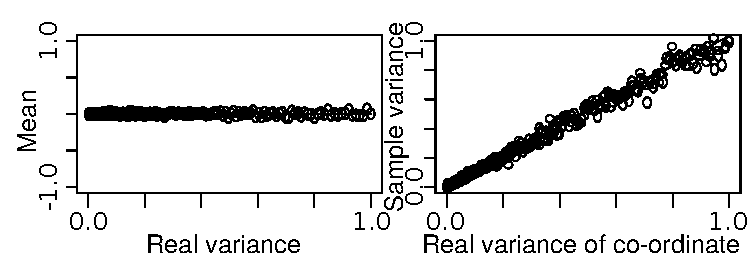
\includegraphics[width=5in]{images/NUTS_comparisons.pdf}
  \caption{Sample Variance against the Real Variance of a multivariate gaussian in 150 dimensions with 1000 samples using NUTS with RStan}
\end{figure}
\subsection{Normal mixture models: Alphabets and EM}
To illustrate HMC, we constructed densities that resemble letters of the alphabets (upper and lower case with ``?" and ``!"). We constructed the densities automatically by applying the EM algorithm on the parameters of the mixture of Gaussians (where the number of mixture was manually tuned) using the R package ``mixtools'' and images of the characters. By specifying a word into our package ``abcHMC", it will simulate samples using HMC from a mixture of bivariate Gaussians, where each letter has the same weights and each letter contains a mixture of bivariate Gaussians found from the EM algorithm. Instead of simulating directly from the density, each mixture in each letter was chosen with probability equal to their weights before simulation with HMC, this is because of the multi-modality of the density. This is still a problem for most MCMC methods, including HMC (see \cite{neal} for tempering methods). Below is the word ``OxWaSP" using 1500 samples from HMC ($\epsilon=0.05$, $L=60$) and similarly for random Walk Metropolis which uses a uniform proposal without thinning. Because it is simulated by through the weights, Metropolis in fact performs equally well when thinning of 15 is used.
\begin{figure}[H]
\center
  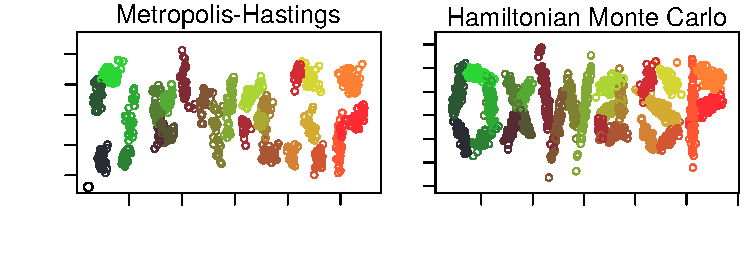
\includegraphics[width=5in]{images/oxwasp.pdf}
  \caption{1500 Samples of mixture of bivariate gaussians with parameters chosen by the EM algorithm, where the different colours corresponds to a different mixture of the gaussian}
\end{figure}

\noindent Our R package consists of 3 separate functions and one dataset.
The dataset, $letter.models$, is stored as a list with 54 elements representing each of the 26 letters of the alphabet in upper and lower case along with the punctuation marks, ``?", and ``!". For each entry there is stored the means, covariances, and mixing proportions of the Gaussian mixture models fitted to represent this character.
\\
\\
The function ``HMC" generates a random sample from a given probability distribution using Hamiltonian Monte Carlo. This function takes as arguments: total.samples, the number of samples you would like generated; q.density, the probability distribution you would like to sample from; diff.density the derivative of the probability density of interest; M, the mass vector; q, the initial value for the `position' in Hamiltonian dynamics; epsilon, the step size to be used in the leapfrog; L, the number of steps to be used in the leapfrog; burnin, the number of iterations of burn-in; output (1 or 0), whether the function should report progress and descriptive statistics on the simulated sample.
\\
\\
The function ``WordForm" simply recodes a single word to specify each letter's position within the letter.models dataset. It takes as input a single word as a character string.
The function ``WordPrint" takes a word and simulates from a probability distribution whose density resembles that word. It takes as inputs word, a character string; and samples, the number of draws which should be made from the distribution. This sampling is done using the HMC function above.
\pagebreak
\begin{thebibliography}{9}

\bibitem{neal}
  Neal R.M.,
  \emph{MCMC using Hamiltonian dynamics},
  Chapter 5 of the Handbook of Markov Chain Monte Carlo,
  2012.
  
\bibitem{duane}
  Duane,S., Kennedy,A.D., Pendleton,B.J., \& Roweth,D.,
  \emph{Hybrid Monte Carlo }
  Physics Letters B, 195(2) 216-222, 1987.

\bibitem{NUTS}
  Hoffman,M.D., Gelman,A.,
  arXiv:1111.4246v1.
  
\bibitem{rstan}
  RStan, \url{http://mc-stan.org/interfaces/rstan.html}

\end{thebibliography}
\end{document}
